% Options for packages loaded elsewhere
\PassOptionsToPackage{unicode}{hyperref}
\PassOptionsToPackage{hyphens}{url}
%
\documentclass[
]{book}
\usepackage{amsmath,amssymb}
\usepackage{iftex}
\ifPDFTeX
  \usepackage[T1]{fontenc}
  \usepackage[utf8]{inputenc}
  \usepackage{textcomp} % provide euro and other symbols
\else % if luatex or xetex
  \usepackage{unicode-math} % this also loads fontspec
  \defaultfontfeatures{Scale=MatchLowercase}
  \defaultfontfeatures[\rmfamily]{Ligatures=TeX,Scale=1}
\fi
\usepackage{lmodern}
\ifPDFTeX\else
  % xetex/luatex font selection
\fi
% Use upquote if available, for straight quotes in verbatim environments
\IfFileExists{upquote.sty}{\usepackage{upquote}}{}
\IfFileExists{microtype.sty}{% use microtype if available
  \usepackage[]{microtype}
  \UseMicrotypeSet[protrusion]{basicmath} % disable protrusion for tt fonts
}{}
\makeatletter
\@ifundefined{KOMAClassName}{% if non-KOMA class
  \IfFileExists{parskip.sty}{%
    \usepackage{parskip}
  }{% else
    \setlength{\parindent}{0pt}
    \setlength{\parskip}{6pt plus 2pt minus 1pt}}
}{% if KOMA class
  \KOMAoptions{parskip=half}}
\makeatother
\usepackage{xcolor}
\usepackage{color}
\usepackage{fancyvrb}
\newcommand{\VerbBar}{|}
\newcommand{\VERB}{\Verb[commandchars=\\\{\}]}
\DefineVerbatimEnvironment{Highlighting}{Verbatim}{commandchars=\\\{\}}
% Add ',fontsize=\small' for more characters per line
\usepackage{framed}
\definecolor{shadecolor}{RGB}{248,248,248}
\newenvironment{Shaded}{\begin{snugshade}}{\end{snugshade}}
\newcommand{\AlertTok}[1]{\textcolor[rgb]{0.94,0.16,0.16}{#1}}
\newcommand{\AnnotationTok}[1]{\textcolor[rgb]{0.56,0.35,0.01}{\textbf{\textit{#1}}}}
\newcommand{\AttributeTok}[1]{\textcolor[rgb]{0.13,0.29,0.53}{#1}}
\newcommand{\BaseNTok}[1]{\textcolor[rgb]{0.00,0.00,0.81}{#1}}
\newcommand{\BuiltInTok}[1]{#1}
\newcommand{\CharTok}[1]{\textcolor[rgb]{0.31,0.60,0.02}{#1}}
\newcommand{\CommentTok}[1]{\textcolor[rgb]{0.56,0.35,0.01}{\textit{#1}}}
\newcommand{\CommentVarTok}[1]{\textcolor[rgb]{0.56,0.35,0.01}{\textbf{\textit{#1}}}}
\newcommand{\ConstantTok}[1]{\textcolor[rgb]{0.56,0.35,0.01}{#1}}
\newcommand{\ControlFlowTok}[1]{\textcolor[rgb]{0.13,0.29,0.53}{\textbf{#1}}}
\newcommand{\DataTypeTok}[1]{\textcolor[rgb]{0.13,0.29,0.53}{#1}}
\newcommand{\DecValTok}[1]{\textcolor[rgb]{0.00,0.00,0.81}{#1}}
\newcommand{\DocumentationTok}[1]{\textcolor[rgb]{0.56,0.35,0.01}{\textbf{\textit{#1}}}}
\newcommand{\ErrorTok}[1]{\textcolor[rgb]{0.64,0.00,0.00}{\textbf{#1}}}
\newcommand{\ExtensionTok}[1]{#1}
\newcommand{\FloatTok}[1]{\textcolor[rgb]{0.00,0.00,0.81}{#1}}
\newcommand{\FunctionTok}[1]{\textcolor[rgb]{0.13,0.29,0.53}{\textbf{#1}}}
\newcommand{\ImportTok}[1]{#1}
\newcommand{\InformationTok}[1]{\textcolor[rgb]{0.56,0.35,0.01}{\textbf{\textit{#1}}}}
\newcommand{\KeywordTok}[1]{\textcolor[rgb]{0.13,0.29,0.53}{\textbf{#1}}}
\newcommand{\NormalTok}[1]{#1}
\newcommand{\OperatorTok}[1]{\textcolor[rgb]{0.81,0.36,0.00}{\textbf{#1}}}
\newcommand{\OtherTok}[1]{\textcolor[rgb]{0.56,0.35,0.01}{#1}}
\newcommand{\PreprocessorTok}[1]{\textcolor[rgb]{0.56,0.35,0.01}{\textit{#1}}}
\newcommand{\RegionMarkerTok}[1]{#1}
\newcommand{\SpecialCharTok}[1]{\textcolor[rgb]{0.81,0.36,0.00}{\textbf{#1}}}
\newcommand{\SpecialStringTok}[1]{\textcolor[rgb]{0.31,0.60,0.02}{#1}}
\newcommand{\StringTok}[1]{\textcolor[rgb]{0.31,0.60,0.02}{#1}}
\newcommand{\VariableTok}[1]{\textcolor[rgb]{0.00,0.00,0.00}{#1}}
\newcommand{\VerbatimStringTok}[1]{\textcolor[rgb]{0.31,0.60,0.02}{#1}}
\newcommand{\WarningTok}[1]{\textcolor[rgb]{0.56,0.35,0.01}{\textbf{\textit{#1}}}}
\usepackage{longtable,booktabs,array}
\usepackage{calc} % for calculating minipage widths
% Correct order of tables after \paragraph or \subparagraph
\usepackage{etoolbox}
\makeatletter
\patchcmd\longtable{\par}{\if@noskipsec\mbox{}\fi\par}{}{}
\makeatother
% Allow footnotes in longtable head/foot
\IfFileExists{footnotehyper.sty}{\usepackage{footnotehyper}}{\usepackage{footnote}}
\makesavenoteenv{longtable}
\usepackage{graphicx}
\makeatletter
\def\maxwidth{\ifdim\Gin@nat@width>\linewidth\linewidth\else\Gin@nat@width\fi}
\def\maxheight{\ifdim\Gin@nat@height>\textheight\textheight\else\Gin@nat@height\fi}
\makeatother
% Scale images if necessary, so that they will not overflow the page
% margins by default, and it is still possible to overwrite the defaults
% using explicit options in \includegraphics[width, height, ...]{}
\setkeys{Gin}{width=\maxwidth,height=\maxheight,keepaspectratio}
% Set default figure placement to htbp
\makeatletter
\def\fps@figure{htbp}
\makeatother
\setlength{\emergencystretch}{3em} % prevent overfull lines
\providecommand{\tightlist}{%
  \setlength{\itemsep}{0pt}\setlength{\parskip}{0pt}}
\setcounter{secnumdepth}{5}
\usepackage{booktabs}
\ifLuaTeX
  \usepackage{selnolig}  % disable illegal ligatures
\fi
\usepackage[]{natbib}
\bibliographystyle{plainnat}
\usepackage{bookmark}
\IfFileExists{xurl.sty}{\usepackage{xurl}}{} % add URL line breaks if available
\urlstyle{same}
\hypersetup{
  pdftitle={A Minimal Book Example},
  pdfauthor={John Doe},
  hidelinks,
  pdfcreator={LaTeX via pandoc}}

\title{A Minimal Book Example}
\author{John Doe}
\date{2024-12-21}

\begin{document}
\maketitle

{
\setcounter{tocdepth}{1}
\tableofcontents
}
\chapter{About}\label{about}

This is a \emph{sample} book written in \textbf{Markdown}. You can use anything that Pandoc's Markdown supports; for example, a math equation \(a^2 + b^2 = c^2\).

\section{Usage}\label{usage}

Each \textbf{bookdown} chapter is an .Rmd file, and each .Rmd file can contain one (and only one) chapter. A chapter \emph{must} start with a first-level heading: \texttt{\#\ A\ good\ chapter}, and can contain one (and only one) first-level heading.

Use second-level and higher headings within chapters like: \texttt{\#\#\ A\ short\ section} or \texttt{\#\#\#\ An\ even\ shorter\ section}.

The \texttt{index.Rmd} file is required, and is also your first book chapter. It will be the homepage when you render the book.

\section{Render book}\label{render-book}

You can render the HTML version of this example book without changing anything:

\begin{enumerate}
\def\labelenumi{\arabic{enumi}.}
\item
  Find the \textbf{Build} pane in the RStudio IDE, and
\item
  Click on \textbf{Build Book}, then select your output format, or select ``All formats'' if you'd like to use multiple formats from the same book source files.
\end{enumerate}

Or build the book from the R console:

\begin{Shaded}
\begin{Highlighting}[]
\NormalTok{bookdown}\SpecialCharTok{::}\FunctionTok{render\_book}\NormalTok{()}
\end{Highlighting}
\end{Shaded}

To render this example to PDF as a \texttt{bookdown::pdf\_book}, you'll need to install XeLaTeX. You are recommended to install TinyTeX (which includes XeLaTeX): \url{https://yihui.org/tinytex/}.

\section{Preview book}\label{preview-book}

As you work, you may start a local server to live preview this HTML book. This preview will update as you edit the book when you save individual .Rmd files. You can start the server in a work session by using the RStudio add-in ``Preview book'', or from the R console:

\begin{Shaded}
\begin{Highlighting}[]
\NormalTok{bookdown}\SpecialCharTok{::}\FunctionTok{serve\_book}\NormalTok{()}
\end{Highlighting}
\end{Shaded}

\chapter{Hello bookdown}\label{hello-bookdown}

All chapters start with a first-level heading followed by your chapter title, like the line above. There should be only one first-level heading (\texttt{\#}) per .Rmd file.

\section{A section}\label{a-section}

All chapter sections start with a second-level (\texttt{\#\#}) or higher heading followed by your section title, like the sections above and below here. You can have as many as you want within a chapter.

\subsection*{An unnumbered section}\label{an-unnumbered-section}
\addcontentsline{toc}{subsection}{An unnumbered section}

Chapters and sections are numbered by default. To un-number a heading, add a \texttt{\{.unnumbered\}} or the shorter \texttt{\{-\}} at the end of the heading, like in this section.

\chapter{Install tidymass shiny APP}\label{install-tidymass-shiny-app}

\section{R package}\label{r-package}

You can find the source code of the package \href{https://github.com/tidymass/tidymass_shiny}{here}.

Use the below code to install the package.

\begin{Shaded}
\begin{Highlighting}[]
\DocumentationTok{\#\#\textgreater{} for chinese users:}
\DocumentationTok{\#\#\textgreater{} options("repos" = c(CRAN="https://mirrors.tuna.tsinghua.edu.cn/CRAN/"))}
\DocumentationTok{\#\#\textgreater{} options(BioC\_mirror="https://mirrors.westlake.edu.cn/bioconductor")}


\ControlFlowTok{if}\NormalTok{ (}\SpecialCharTok{!}\FunctionTok{require}\NormalTok{(}\StringTok{\textquotesingle{}remotes\textquotesingle{}}\NormalTok{)) }\FunctionTok{install.packages}\NormalTok{(}\StringTok{\textquotesingle{}remotes\textquotesingle{}}\NormalTok{);}
\ControlFlowTok{if}\NormalTok{ (}\SpecialCharTok{!}\FunctionTok{require}\NormalTok{(}\StringTok{\textquotesingle{}tidyverse\textquotesingle{}}\NormalTok{)) }\FunctionTok{install.packages}\NormalTok{(}\StringTok{\textquotesingle{}tidyverse\textquotesingle{}}\NormalTok{);}
\ControlFlowTok{if}\NormalTok{ (}\SpecialCharTok{!}\FunctionTok{require}\NormalTok{(}\StringTok{\textquotesingle{}tidymass\textquotesingle{}}\NormalTok{)) \{}
  \FunctionTok{source}\NormalTok{(}\StringTok{"https://www.tidymass.org/tidymass{-}packages/install\_tidymass.txt"}\NormalTok{);}
  \FunctionTok{install\_tidymass}\NormalTok{(}\AttributeTok{from =} \StringTok{"tidymass.org"}\NormalTok{)}
\NormalTok{\};}
\ControlFlowTok{if}\NormalTok{ (}\SpecialCharTok{!}\FunctionTok{require}\NormalTok{(}\StringTok{\textquotesingle{}shinyFiles\textquotesingle{}}\NormalTok{)) remotes}\SpecialCharTok{::}\FunctionTok{install\_github}\NormalTok{(}\StringTok{\textquotesingle{}thomasp85/shinyFiles\textquotesingle{}}\NormalTok{);}
\ControlFlowTok{if}\NormalTok{ (}\SpecialCharTok{!}\FunctionTok{require}\NormalTok{(}\StringTok{\textquotesingle{}shinyWidgets\textquotesingle{}}\NormalTok{)) remotes}\SpecialCharTok{::}\FunctionTok{install\_github}\NormalTok{(}\StringTok{"dreamRs/shinyWidgets"}\NormalTok{);}
\ControlFlowTok{if}\NormalTok{ (}\SpecialCharTok{!}\FunctionTok{require}\NormalTok{(}\StringTok{\textquotesingle{}shiny\textquotesingle{}}\NormalTok{)) }\FunctionTok{install.packages}\NormalTok{(}\StringTok{\textquotesingle{}shiny\textquotesingle{}}\NormalTok{);}
\ControlFlowTok{if}\NormalTok{ (}\SpecialCharTok{!}\FunctionTok{require}\NormalTok{(}\StringTok{\textquotesingle{}bsicons\textquotesingle{}}\NormalTok{)) }\FunctionTok{install.packages}\NormalTok{(}\StringTok{\textquotesingle{}bsicons\textquotesingle{}}\NormalTok{);}
\ControlFlowTok{if}\NormalTok{ (}\SpecialCharTok{!}\FunctionTok{require}\NormalTok{(}\StringTok{\textquotesingle{}bslib\textquotesingle{}}\NormalTok{)) }\FunctionTok{install.packages}\NormalTok{(}\StringTok{\textquotesingle{}bslib\textquotesingle{}}\NormalTok{);}
\ControlFlowTok{if}\NormalTok{ (}\SpecialCharTok{!}\FunctionTok{require}\NormalTok{(}\StringTok{\textquotesingle{}plotly\textquotesingle{}}\NormalTok{)) }\FunctionTok{install.packages}\NormalTok{(}\StringTok{\textquotesingle{}plotly\textquotesingle{}}\NormalTok{);}
\ControlFlowTok{if}\NormalTok{ (}\SpecialCharTok{!}\FunctionTok{require}\NormalTok{(}\StringTok{\textquotesingle{}colourpicker\textquotesingle{}}\NormalTok{)) }\FunctionTok{install.packages}\NormalTok{(}\StringTok{\textquotesingle{}colourpicker\textquotesingle{}}\NormalTok{);}
\ControlFlowTok{if}\NormalTok{ (}\SpecialCharTok{!}\FunctionTok{require}\NormalTok{(}\StringTok{\textquotesingle{}plantmdb\textquotesingle{}}\NormalTok{)) remotes}\SpecialCharTok{::}\FunctionTok{install\_github}\NormalTok{(}\StringTok{"xuebinzhang{-}lab/plantmdb"}\NormalTok{)  }\DocumentationTok{\#\# plant metabolomics database. for test use.}
\ControlFlowTok{if}\NormalTok{ (}\SpecialCharTok{!}\FunctionTok{require}\NormalTok{(}\StringTok{\textquotesingle{}tidymassshiny\textquotesingle{}}\NormalTok{)) remotes}\SpecialCharTok{::}\FunctionTok{install\_github}\NormalTok{(}\StringTok{\textquotesingle{}tidymass/tidymass\_shiny\textquotesingle{}}\NormalTok{)}
\end{Highlighting}
\end{Shaded}

\section{Start tidymass shiny APP}\label{start-tidymass-shiny-app}

\begin{Shaded}
\begin{Highlighting}[]
\FunctionTok{run\_tidymass\_shiny}\NormalTok{()}
\end{Highlighting}
\end{Shaded}

The tidymass shiny App will start like below shows:

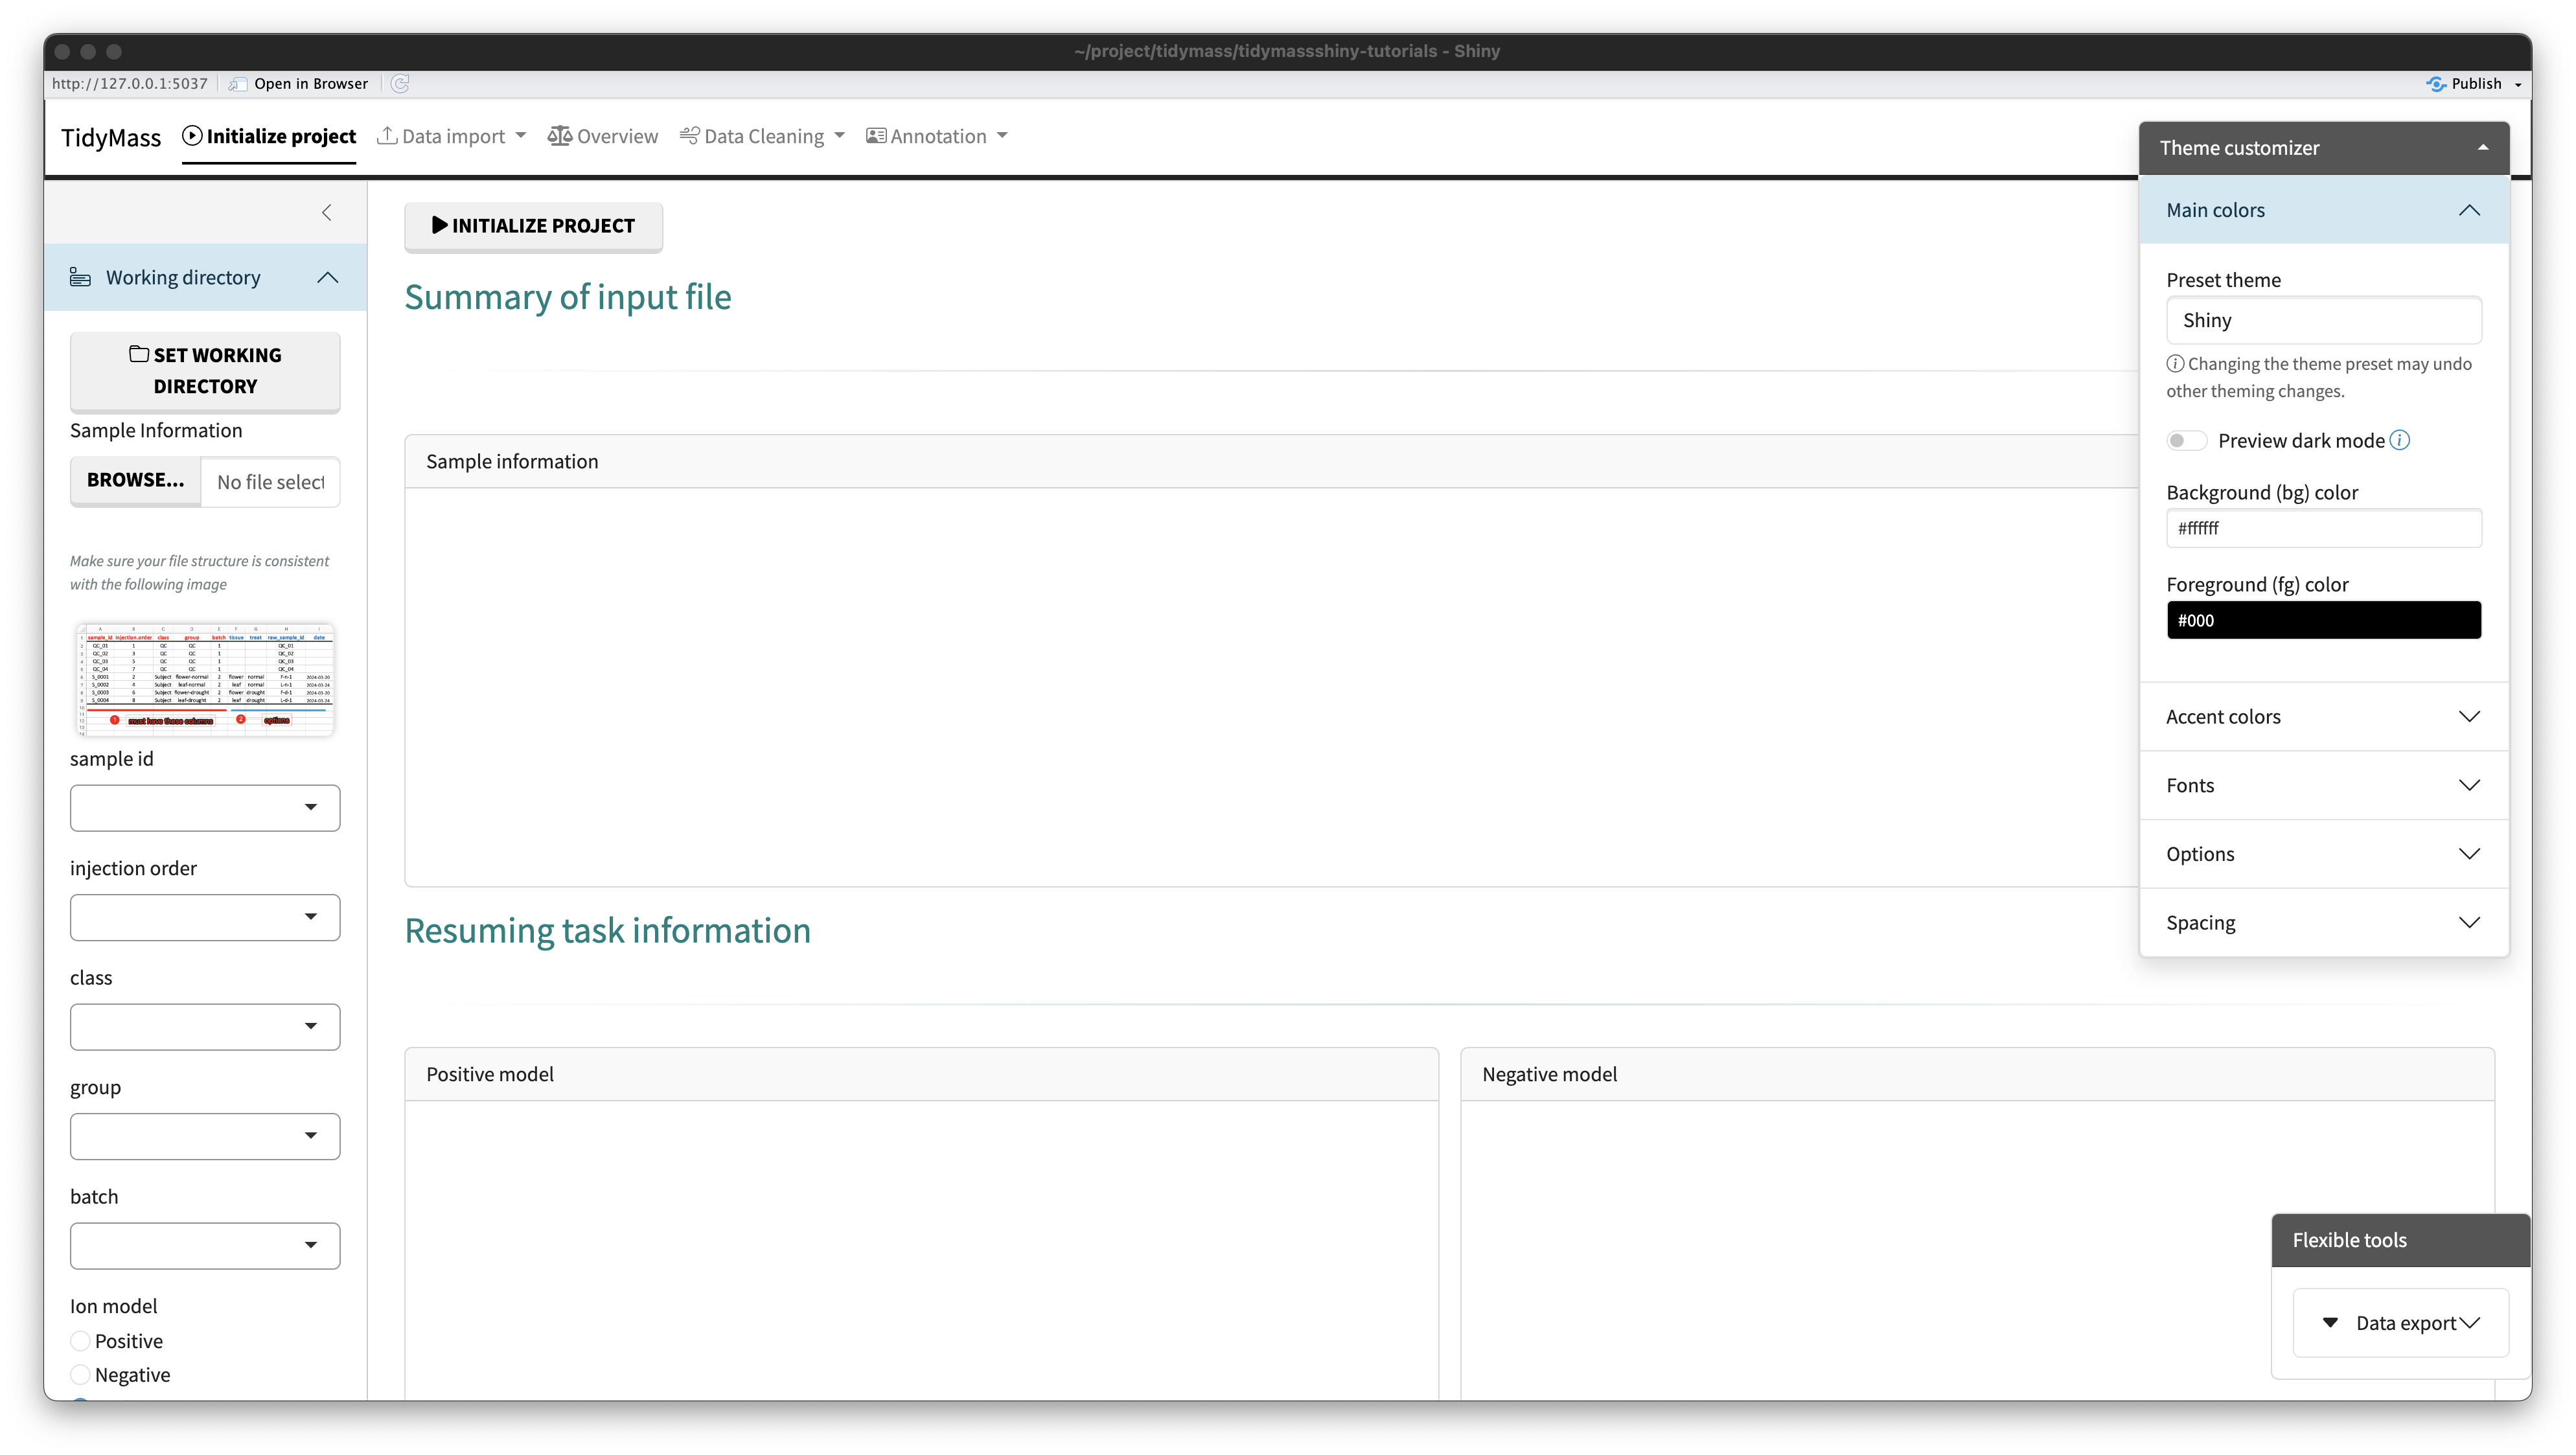
\includegraphics{figures/figure1.png}

\chapter{Start one project}\label{start-one-project}

\section{R package}\label{r-package-1}

1234

xiaotao shen test

123

  \bibliography{book.bib,packages.bib}

\end{document}
